\documentclass{article}

% Language setting
\usepackage[italian]{babel}

% Set page size and margins
\usepackage[a4paper,top=2cm,bottom=2cm,left=2cm,right=2cm,marginparwidth=1.75cm]{geometry}

% Useful packages
\usepackage{amsmath}
\usepackage{amssymb} 
\usepackage{comment}    %scrivere commenti multirighe
\usepackage{graphicx}
\usepackage{microtype}
\usepackage[colorlinks=true,allcolors=teal]{hyperref}
\usepackage{xcolor}

% set san-serif font for all the document
\renewcommand{\familydefault}{\sfdefault}
% text style to create a code snippet
\definecolor{codegray}{gray}{0.9}
\newcommand{\code}[1]{\colorbox{codegray}{\texttt{#1}}}

% Title
\title{\textbf{Relazione Progetto di Calcolo Numerico}}
\author{Benatti Alice, Manuelli Matteo, Qayyum Shahbaz Ali}
\date{gennaio 2022}

\begin{document}
\maketitle

% Summary
\tableofcontents

\newpage
% All content
\begin{comment}
Relazione

1. Riportare e commentare i risultati ottenuti nei punti 2. 3. (e 4.) 
su un immagine del set creato e su altre due immagini in bianco e nero 
(fotografiche/mediche/astronomiche)
2. Riportare delle tabelle con le misure di PSNR e MSE ottenute al 
variare dei parametri (dimensione kernel, valore di sigma, la 
deviazione standard del rumore, il parametro di regolarizzazione). 
3. Calcolare sull’intero set di immagini medie e deviazione standard 
delle metriche per alcuni valori fissati dei parametri.  
4. Analizzare su 2 esecuzioni le proprietà dei metodi numerici 
utilizzati (gradiente coniugato e gradiente) in termini di numero di 
iterazioni, andamento dell’errore, della funzione obiettivo, norma del 
gradiente. 
\end{comment}

L'obiettivo del progetto è comprendere e mettere in atto metodi per la ricostruizione, o recupero, di 
immagini blurrate, lavorando su problemi test, ovvero abbiamo generato corrotte da un rumore 
Gaussiano applicandolo ad un set di immagini pulite in modo tale da analizzare il problema. 

Inizialmente verrà analizzata l'immagine \code{data.camera()} importata da
\code{skimage}, successivamente verranno analizzate 8 immagini con oggetti geometrici
 di colore uniforme su sfondo nero, realizzate da noi.

Il problema di deblur consiste nella ricostruzione di un immagine a partire da un dato acquisito
 mediante il seguente modello:
\[b=Ax+\eta\]
dove $b$ rappresenta l'immagine corrotta, $x$ l'immagine originale che vogliamo ricostruire, $A$ 
l'operatore che applica il blur Gaussiano ed $\eta$ il rumore additivo con distribuzione Gaussiana di
 media 0 e deviazione standard $\sigma$.

Per svolgere il progetto si farà uso dei moduli \code{numpy}, \code{skimage} e \code{matplotlib}
utilizzando il linguaggio Python.

Affinché risultino chiari i valori a cui andremo a riferirci nella relazione, bisogna tenere ben presente 
il significato di questi due parametri. 

\textbf{PSNR (Peak Signal to Noise Ratio):} Misura la qualità di un immagine ricostruita rispetto all'immagine 
originale, la formula per calcolarlo è la seguente: \[PSNR = log_{10}(\frac{max\;x^\ast}{\sqrt{MSE}})\]

\textbf{MSE (Mean Squared Error):}  Con la sigla ci riferiamo all'errore quadratico medio ed è così ottenuto:
 \[MSE = \sqrt[2]{\frac{\sum_{i=1}^n\sum_{j=1}(x^{\ast}_{ij}-x_{ij})}{nm}}\]

I due valori sono inversamente proposizionali; più è alto il PSNR e basso l'MSE, più l'immagine sarà 
simile all'immagine originale. il PSNR dipende dall'MSE.

\textbf{Deviazione standard:} indica quanto sono distribuiti i dati rispetto alla loro media: 
un valore piccolo indica che i dati sono "ammassati" intorno al valore medio, 
mentre un valore grande indica che i dati sono distribuiti lungo tutto il grafico.

\begin{figure}[H]\centering
	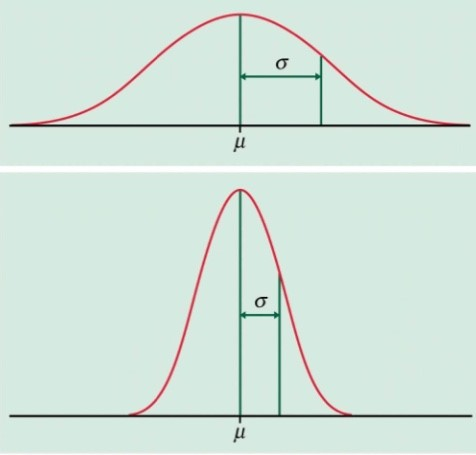
\includegraphics[width=0.3\textwidth]{MANCANTI/deviazione standard.jpg}
	\caption{Distrubuzione valori rispetto ad un valore medio}
\end{figure}
\section{Ricostruzione di un immagine rispetto una versione corrotta}
Una possibile ricostruzione dell'immagine originale $x$ partendo dall'immagine corrotta $b$ è la soluzione naive data dal minimo del seguente problema di ottimizzazione:
\[x^* = \arg\min_x \frac{1}{2} ||Ax - b||_2^2\]

Nell'analisi delle immagini ricostruite useremo $\sigma=1$ dimensione $7\times 7$ come valore standard.
%! immagine grafico  mg vs mgc

Abbiamo mostrato questi due grafici sovrastanti perché si evince che all'aumentare del numero delle 
iterazioni l'immagine ricavata si allontana dalla sua versione originale poiché è presente una deviazione. 



\end{document}